\chapter{RNA Motifs}
\label{motifs} 
\bibliographystyle{nar}
As mentioned in  Chapter 2 the most common  perspectives for RNA motif
recognition  and  discovery are  the  atom  and  bond based  ones, the
rigid-body-based perspective has been  rather unexplored. The two main
questions that we would like to address in this context are:

\begin{enumerate}
\item{Can  the geometric rigid-block  description of  base-pairing and
  base-stacking solve the problem of defining RNA structural motifs?}
\item{Can we use quantities derived  from the 3DNA software package to
  make and automatic  search for a known motif,  for example, the GNRA
  tetraloop motif, and perhaps find unknown motifs?}
\end{enumerate}

We have  started with  the second  question and have  chosen as
workhorse the well known GNRA tetraloop motif. We have also used other
quantities  (e.g.  endocyclic  and  exocyclic base-overlaps)  obtained
with  the 3DNA  \cite{lu2003, lu2008b}  package, and  quantified their
relationship to RNA motifs.

\section{The GNRA Tetraloop}
The  GNRA  motif   was  initially  found  to  be   important  for  the
organization  of  large RNA  structures  like  the  ribosome from  the
context of comparative sequence analysis \cite{woese1990}, that is, it
was seen  that the GNRA  sequence was commonly repeated  among various
organisms, and so were other  tetraloops, but the most abundant one of
all tetraloops in the ribosome is the GNRA one \cite{pardi1991}.


The  GNRA  tetraloop  motif  is   one  of  the  most  well  known  and
characterized motifs in RNA  structures, its description is a typical
case  of the  problem of  RNA motif  definition, for  example,  in the
sequence alone context  a GNRA motif would be one  which follows, in a
consecutive manner, the GNRA pattern, whereas it has been noticed that
there can be GNRA structures which are not consecutive in sequence but
have   the   same    arrangement   of   bases   in   three-dimensional
space \cite{lemieux2006}.






Description and brief survey of the motif.
First  formally  described  by  Woese \cite{woese1990}  in  1990  from
comparative  sequence analysis,  although supossedly  recognized since
1985. First characterized in NMR by Heus and Pardi \cite{heus1991}
Various MD studies.
\cite{depaul2010}


\begin{figure}
\centering 
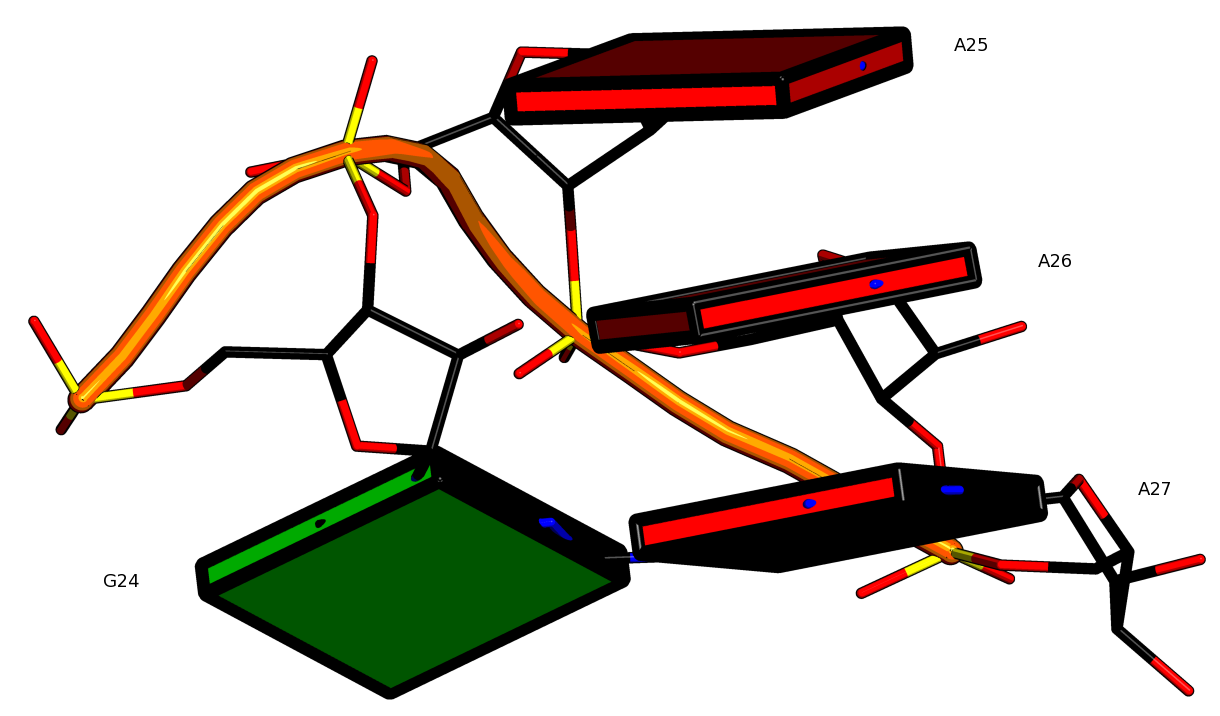
\includegraphics[angle=0, scale=2]{Chapter5/gnra24.png}
\caption{GNRA Tetraloop from the \textit{Azoarcus} group I intron,
  PDB-ID:3iin   \cite{antonioli2010}.}
\end{figure}

We have built an algorithm to search for GNRA motifs, the algortihm is
illustrated in figure such.

The algorithm could take any seed but for now only GNRA. In the future
the aim is to make a database of motif base-step parameters.
The seed  is made  up of known  GNRA structures whose  parameters have
been calculated with 3DNA.
We have taken the mean single stranded base-step parameters in 14 GNRA
tetraloops found  in the 1ffk  for the GN,  NR, RA steps and  put them
into a 3 by 6 matrix. The values can be seen in table:

We  compute the  sum of  the difference  between the  GNRA  matrix and
sequential 3 by six  matrices resulting from the step-parameter output
of 3DNA. With  this score we can find the GNRA  tetraloops given a pdb
file.

In the  RNA ontology consortium (ROC)  meeting of May,  2009 a reduced
dataset        of        RNA        structures        found        at:
\url{https://docs.google.com/Doc?id=dhrmkfmn_13ftpbjcgq}    was   made
available to participants with the  purpose of allowing them to search
for RNA motifs, which would later be compared between groups.

We have started with just a few, five. The results are shown in:

The  algorithm still  falls for  cases  where the  pdb structures  are
non-sequential and  have large jumps  in sequence, or where  there are
more than one  single stranded chain, for example  in 1ffk since there
are two residues which are numbered 90, one in the 23S, and one in the
5S, then it finds a mismatch on the 23S.


%\section{Canonical "Noise"}
%To be able to say anything about motifs it's crucial to get rid of the
%"noise" which is given by the canonical base-pair steps.
%One would think that perhaps  the X3DNA-Parser of Dr. Yurong Xin could
%help  in the  task, but  then, it  can't, because  it's based  on what
%base-pairs  have  been found,  therefore,  it  tells  me about  single
%stranded interactions,  it doesn't tell  me about bases which  are not
%forming interactions and are alone.

%\subsection{3DNA-Parser}
%We started by using Dr. Yurong Xin's 3DNA-Parser hoping that the
%description of the enclosing base pair in the loop, that is, the
%sheared G$\cdot$A, would have a characteristic signature.
%We found that such is not the case. We know from Major et
%al. \cite{lemieux2006} that there should be at least 21 GNRA tetraloops
%in the 23S subunit of rRNA. We used the G2696 N2697 R2698 A2699
%tetraloop as a seed (as can be seen in Figure 1.1) and found out
%that according to Dr. Xin's helical classification the enclosing G is
%classified as $S_{hq}$ and A is classified as $H_{e}$. 

%We then searched all such instances for G$\cdot$A base-pairs and we
%found seven hits, but none were in fact GNRA tetraloops.

\subsection{Overlap Scores} 
We  clustered the  overlap  values  impossing a  cutoff  of values  of
[1-8]. Since a large amount of overlap values are exactly zero (33\%),
so, without the cutoff the zero values "overshadow" the data.
\begin{figure}[htbp]
\centering 
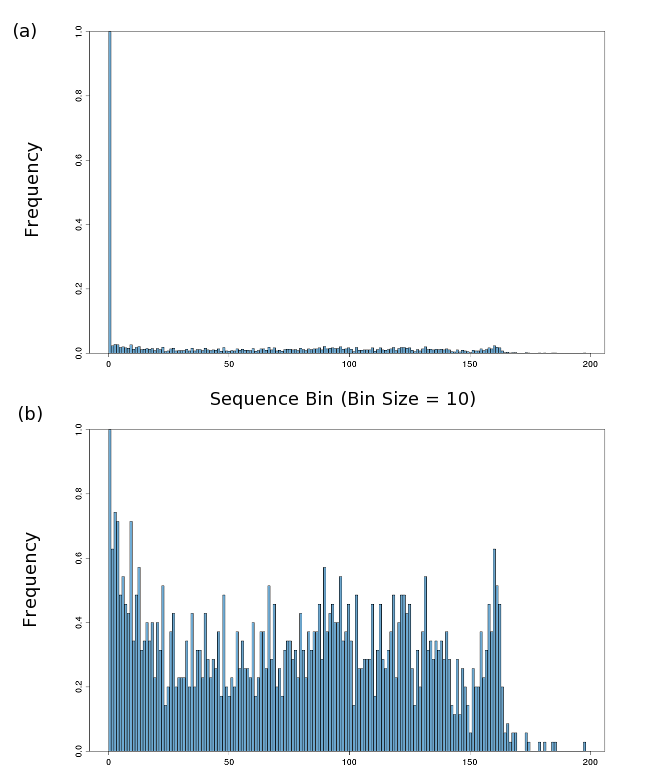
\includegraphics[angle=0, scale=0.8]{Chapter5/histocompare.png}
\caption{Normalized  histograms showing  the  distribution of  overlap
  values  in the  23S subunit  or \textit{Thermus  Thermophilus} rRNA,
  PDB-ID:1jjk.  In  histogram (a)  all  values  are  included, but  in
  histogram (b) only values greater than zero are included. Notice the
  high preponderance  of zero  values, exactly 897  out of a  total of
  2705.}
\end{figure}
For this case we obtained a ``good'' dendrogram as seen in Figure 1.2.
\begin{figure}[htbp]
\centering 
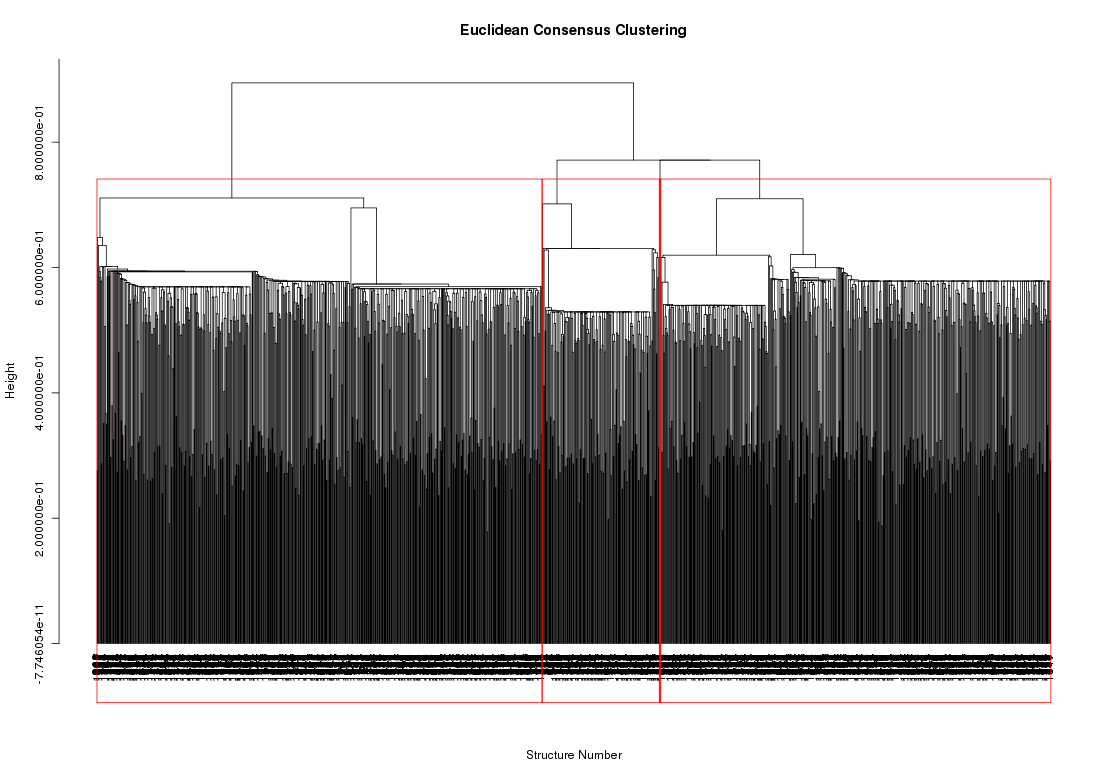
\includegraphics[angle=90, scale=0.6]{Chapter5/eucli_cons.png}
\caption{Dendrogram for consensus clustering  of overlap scores in the
  ribosome.  Zero values filtered out and remaining data normalized.}
\end{figure}

The next  step in this analysis  will be to find  the structures which
correspond  to this  clusters  and superimpose  and  align them  using
Kabsh's algorithm to be able to determine their RMSD's.

Many people  start their  RNA Motif identification  and classification
algorithms by splitting  RNA structures into what is  helical and what
is not,  and then  finding interactions between  these two  groups. We
believe that  we could do  a similar exercise  with 3DNA by  using the
scalar  product   of  helical  axis  vectors  and   once  helical  and
non-helical regions are  found we might be able to  use 3DNA Parser to
look for characteristic interactions.

%\section{Triplets on RNA (comparison to Laing et al.)}

\section{Conclusions}
We  answer  the questions  at  the begining  of  this  chapter in  the
following way:

\begin{enumerate}
\item{\textbf{Q.}  Can   the  geometric  rigid-block   description  of
  base-pairing  and base-stacking  solve the  problem of  defining RNA
  structural motifs?}
\item{\textbf{A.}  The problem  of defining  RNA structural  motifs is
  clearly  more  complicated  than  what  can  be  understood  by  any
  structural  research  methodology  alone.  We have  shown  that  the
  rigid-body parameter view of RNA  can easily automate the process of
  motif  searches  in RNA  atomic  structures,  and  it helps  in  the
  description   of   motifs,    therefore   we   believe   that   this
  characterization should not be ignored by the community and included
  in ontological efforts such as the ROC one.}
\item{\textbf{Q.} Can we use quantities derived from the 3DNA software
  package to make and automatic search for a known motif, for example,
  the GNRA tetraloop motif, and perhaps find unknown motifs?}
\item{\textbf{A.} Yes. by defining seeds from known motifs we can find
new motifs in  the boundaries of known ones  via base-pairs steps. But
we  can also  do  other,  yet simpler,  not  as ``precise''  searches,
e.g. by clustering  the results of base overlaps.  Other searches have
not  been explored  but could  also be  useful, for  example exploring
helical  parameters like x-displacement,  y-displacement, inclination,
tip.} 
\end{enumerate}

\bibliography{biblio}

